\documentclass[12pt]{article}
\usepackage{amsmath}
\usepackage{tikz}
\usepackage{color}
\usetikzlibrary{arrows}
\tikzset{
    vertex/.style = {
        circle,
        draw,
        outer sep = 3pt,
        inner sep = 3pt,
    },edge/.style = {->,> = latex'}
}
\usepackage{amssymb}

\begin{document}

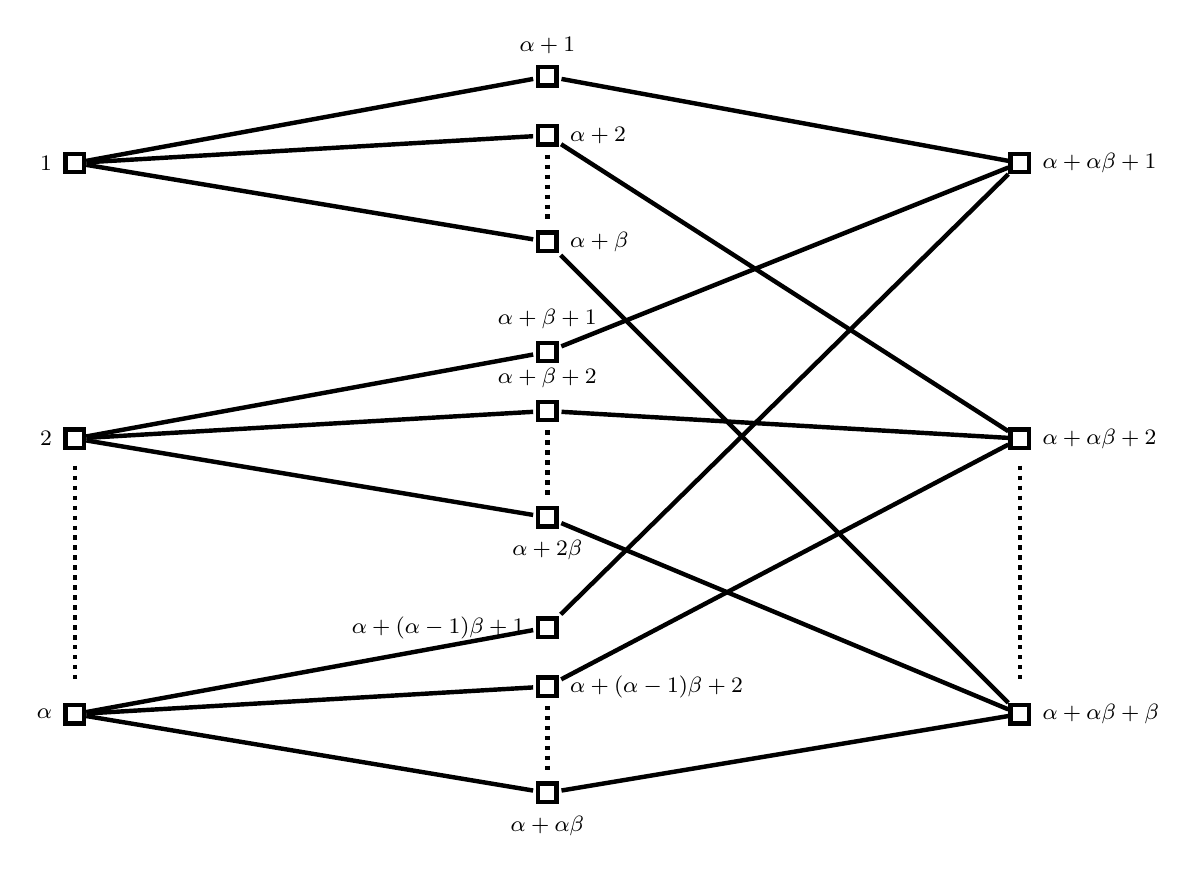
\begin{tikzpicture}[shorten >=1pt, auto, node distance=3cm, ultra thick,
   node_style/.style={circle,draw=black,fill=white !20!,font=\sffamily\Large\bfseries},
   edge_style/.style={draw=black, ultra thick}]
\node[label=left:\footnotesize$1$,draw] (1) at  (0,0) {};
\node[label=left:\footnotesize$2$,draw] (2) at  (0,-3.5) {};
\node (3) at  (0,-3.7) {};
\node (alpha-1) at  (0,-6.8) {}; 
\node[label=left:\footnotesize$\bf{\alpha}$,draw] (alpha) at  (0,-7) {}; 
\node[label=above:\footnotesize${\alpha+1}$,draw] (alpha+1) at  (6,1.1) {};
\node[label=right:\footnotesize$\alpha+2$,draw] (alpha+2) at  (6,0.35) {};
\node (alpha+3) at  (6,0.25) {};
\node (alpha+beta-1) at  (6,-0.9) {};
\node[label=right:\footnotesize$\alpha+\beta$,draw] (alpha+beta) at  (6,-1) {};
\node[label=above:\footnotesize$\alpha+\beta+1$,draw] (alpha+beta+1) at  (6,-2.4) {};
\node[label=above:\footnotesize$\alpha+\beta+2$,draw] (alpha+beta+2) at  (6,-3.15) {};
\node (alpha+beta+3) at  (6,-3.25) {};
\node (alpha+2beta-1) at  (6,-4.4) {};
\node[label=below:\footnotesize$\alpha+2\beta$,draw] (alpha+2beta) at  (6,-4.5) {};
\node[label=left:\footnotesize$\alpha+(\alpha-1)\beta+1$,draw] (alpha+alpha-1beta+1) at  (6,-5.9) {};
\node[label=right:\footnotesize$\alpha+(\alpha-1)\beta+2$,draw] (alpha+alpha-1beta+2) at  (6,-6.65) {};
\node (alpha+alpha-1beta+3) at  (6,-6.75) {};
\node (alpha+alphabeta-1) at  (6,-7.9) {};
\node[label=below:\footnotesize$\alpha+\alpha\beta$,draw] (alpha+alphabeta) at  (6,-8) {};
\node[label=right:\footnotesize$\alpha+\alpha\beta+1$,draw] (alpha+alphabeta+1) at  (12,0) {};
\node[label=right:\footnotesize$\alpha+\alpha\beta+2$,draw] (alpha+alphabeta+2) at  (12,-3.5) {};
\node (alpha+alphabeta+3) at  (12,-3.7) {};
\node (alpha+alphabeta+beta-1) at  (12,-6.8) {};
\node[label=right:\footnotesize$\alpha+\alpha\beta+\beta$,draw] (alpha+alphabeta+beta) at  (12,-7) {};
\draw  (1) to (alpha+1);
\draw  (1) to (alpha+2);
\draw  (1) to (alpha+beta);
\draw  (2) to (alpha+beta+1);
\draw  (2) to (alpha+beta+2);
\draw  (2) to (alpha+2beta);
\draw  (alpha) to (alpha+alpha-1beta+1);
\draw  (alpha) to (alpha+alpha-1beta+2);
\draw  (alpha) to (alpha+alphabeta);
\draw  (alpha+alphabeta+1) to (alpha+1);
\draw  (alpha+alphabeta+1) to (alpha+beta+1);
\draw  (alpha+alphabeta+1) to (alpha+alpha-1beta+1);
\draw  (alpha+alphabeta+2) to (alpha+2);
\draw  (alpha+alphabeta+2) to (alpha+beta+2);
\draw  (alpha+alphabeta+2) to (alpha+alpha-1beta+2);
\draw  (alpha+alphabeta+beta) to (alpha+beta);
\draw  (alpha+alphabeta+beta) to (alpha+2beta);
\draw  (alpha+alphabeta+beta) to (alpha+alphabeta);
\begin{scope}[dotted]
\draw  (3) to (alpha-1);  
\draw (alpha+3) to (alpha+beta-1);
\draw (alpha+beta+3) to (alpha+2beta-1);
\draw (alpha+alpha-1beta+3) to (alpha+alphabeta-1);
\draw (alpha+alphabeta+3) to (alpha+alphabeta+beta-1);
\end{scope}
\end{tikzpicture}

\end{document}